\subsection{Mancala}


\begin{quote}
``The object of the game is to capture more seeds than one's opponent.
At the beginning of the game, three seeds are placed in each house.
Each player controls the six houses and their seeds on his/her side of the board. His/her score is the number of seeds in the store to his/her right.
Players take turns sowing their seeds. On a turn, the player removes all seeds from one of the houses under his/her control. Moving counter-clockwise, the player drops one seed in each house in turn, including the player's own store but not his/her opponent's.
If the last sown seed lands in the player's store, the player gets an additional move. There is no limit on the number of moves a player can make in his/her turn.
If the last sown seed lands in an empty house owned by the player, and the opposite house contains seeds, both the last seed and the opposite seeds are captured and placed into the player's store.
When one player no longer has any seeds in any of his/her houses, the game ends. The other player moves all remaining seeds to his/her store, and the player with the most seeds in his/her store wins.
It is possible for the game to end in a draw, with 18 seeds each.''
\end{quote} %http://en.wikipedia.org/wiki/Kalah

\begin{figure}
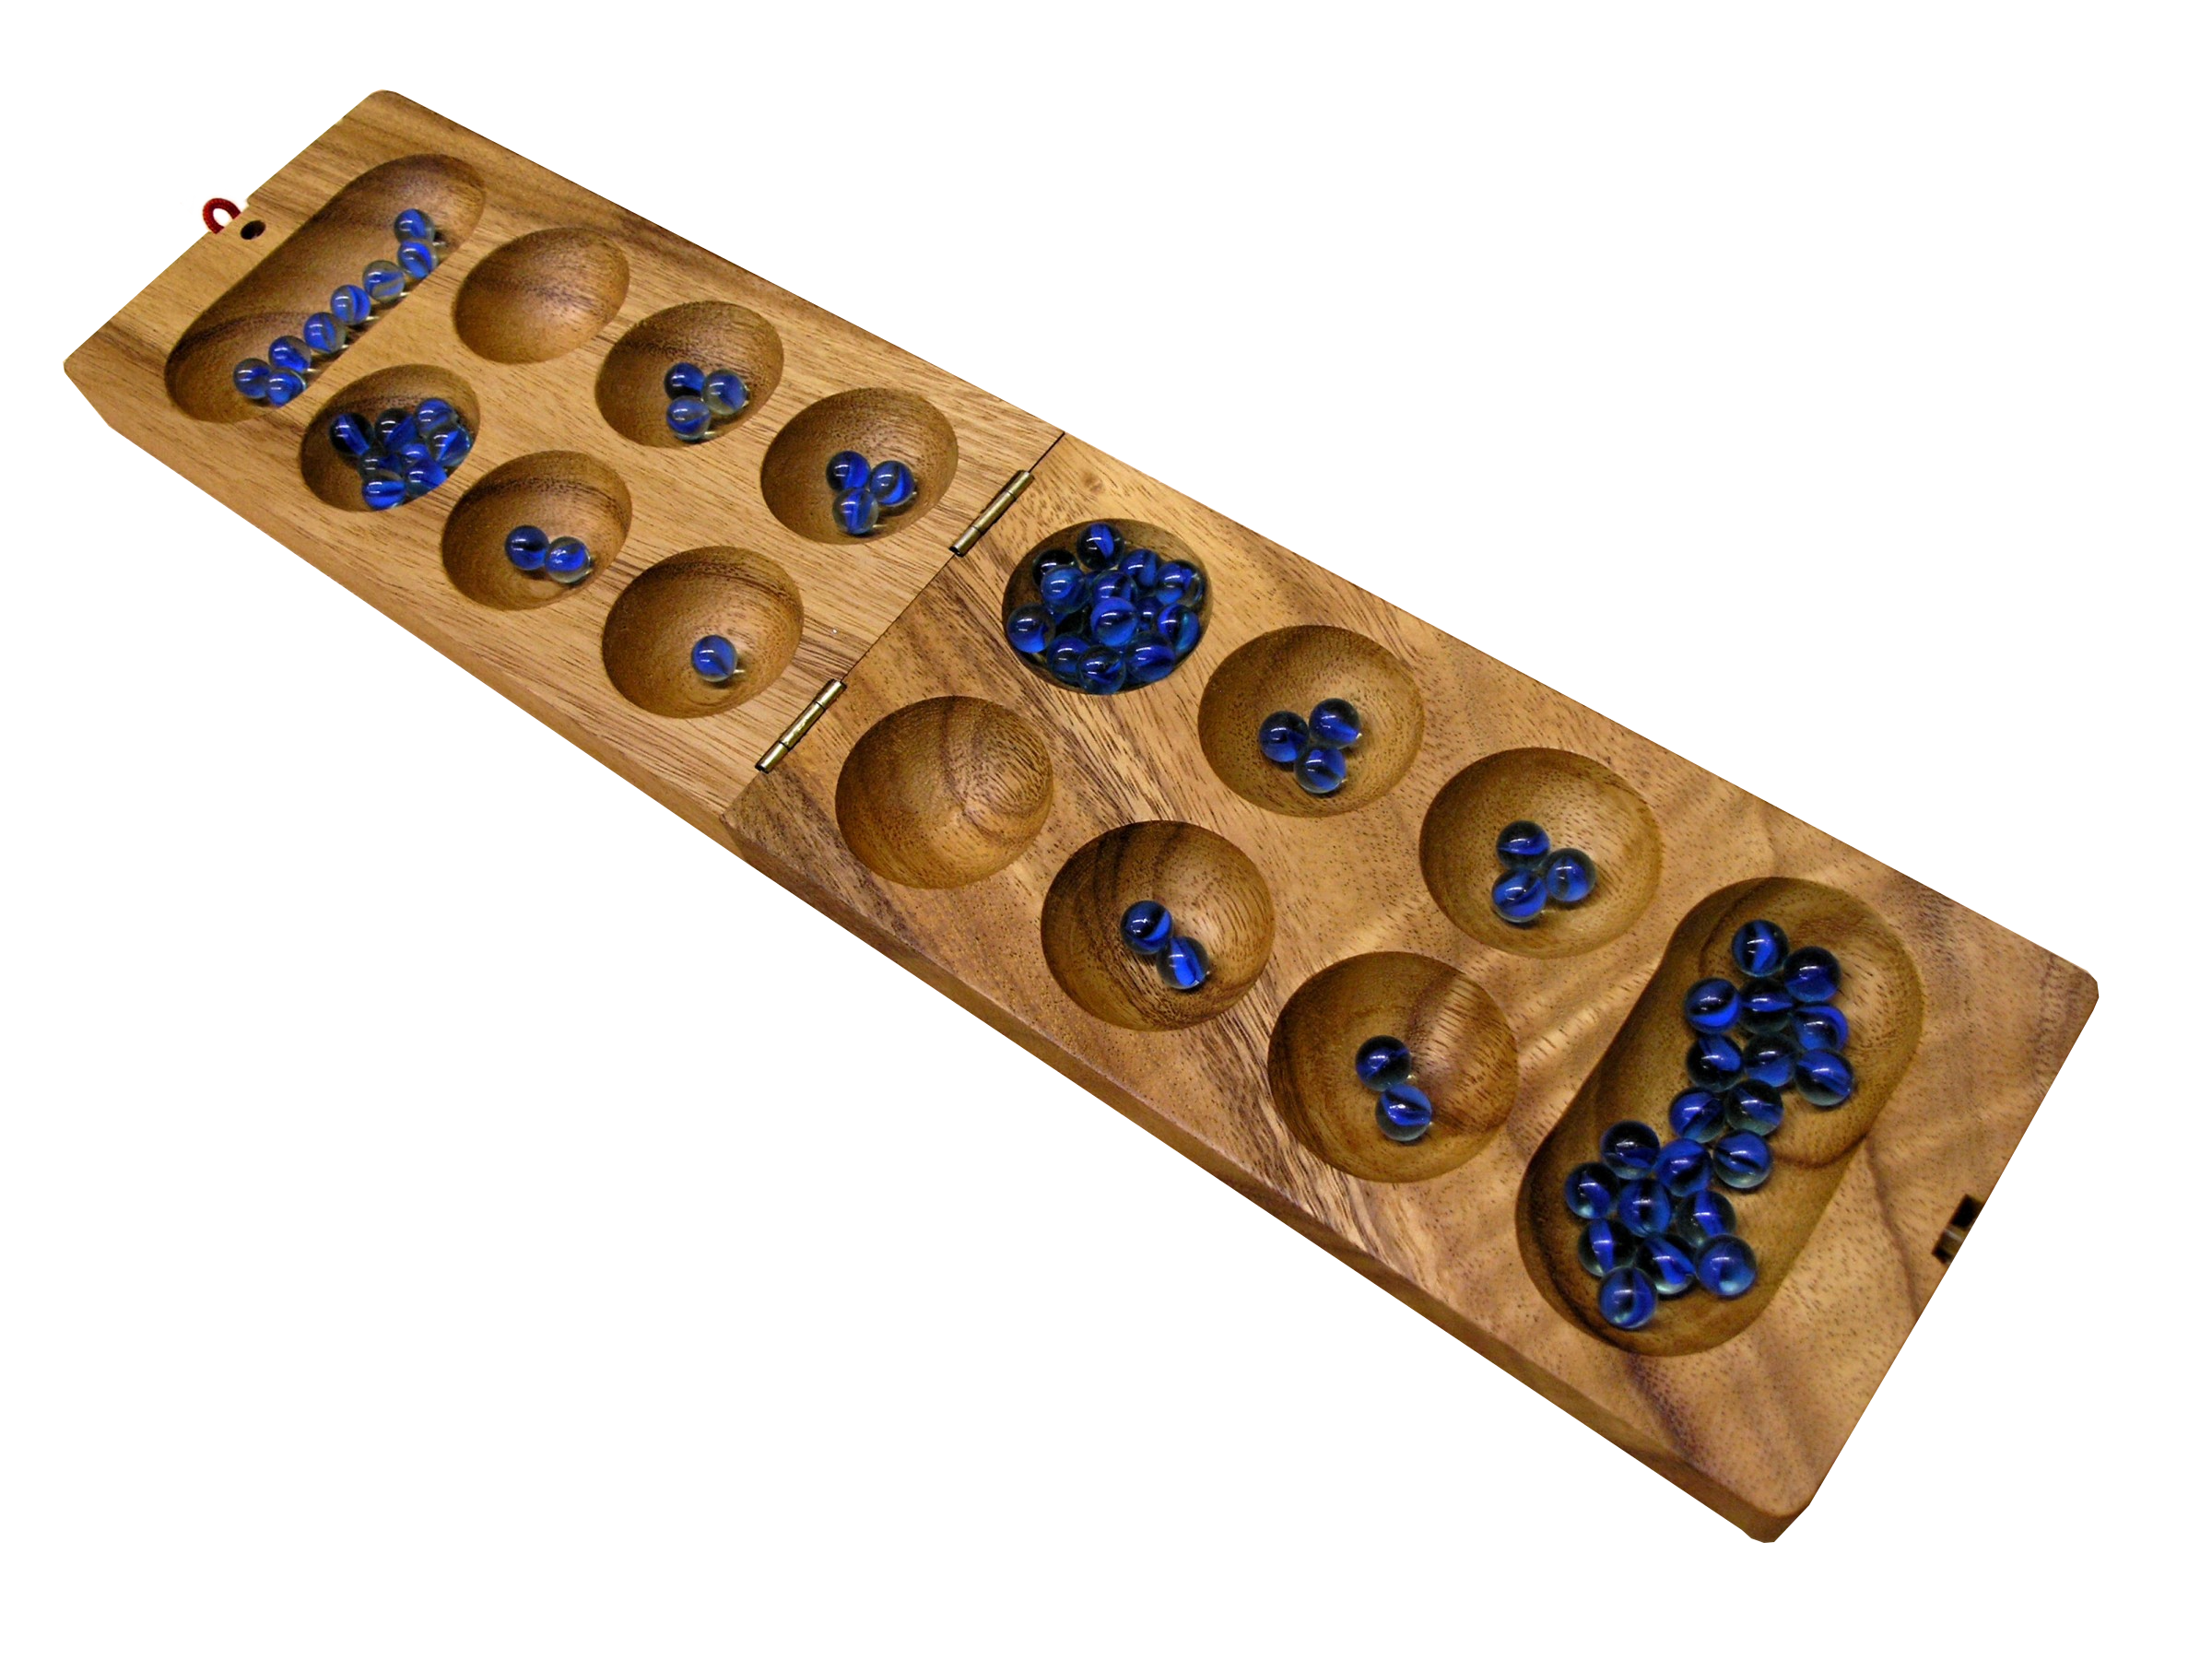
\includegraphics[scale=0.1]{pictures/kalaha.png}
\capt{The board game Kalah}
\end{figure}

When comparing Kalah and the game elements involved to other board games, some interesting requirements for a generic board game programming language able to describe this particulary game arises. The requirements described here consider seeds as pieces and the houses as squares, which makes it easier to compare the requirements of Kalah to the requirements of other board games later.
\begin{itemize}
\item Squares can contain an arbitrary number of pieces
\item Making a move can be considered as simply choosing a square
\item A turn may contain more than one move
	\begin{itemize}
	\item If you do not land on 
	\end{itemize}
\item A square can be related to a player
	\begin{itemize}
	\item A winner is found based on who has most pieces in a special square
	\item On your turn you can only choose a square beloning to you
	\end{itemize}
\item Squares can be related to other squares
	\begin{itemize}
	\item You place pieces on squares counter-clowise
	\item If you place a last piece on an empty square, the nearest square controlled by the opponent is emptied.
	\end{itemize}
\item Only one type of pieces
\end{itemize}
